\documentclass[10pt,a4paper]{article}
\usepackage[utf8]{inputenc}
\usepackage{amsmath}
\usepackage{amsfonts}
\usepackage{amssymb}
\usepackage{geometry}
\usepackage{verbatim}
\usepackage{enumerate}
\usepackage{fancyvrb}
\usepackage{graphicx}
\usepackage{tikz}
\usetikzlibrary{positioning}
\usetikzlibrary{shapes,snakes}
\usepackage[english]{babel}

\geometry{legalpaper, margin=1.5in}

\author{William Schultz}
\begin{document}
\title{Computer Architecture}
\author{William Schultz}
\maketitle

At a high level, any computer can be viewed as consisting of the following abstract components:
\begin{enumerate}
    \item \textbf{Input}
    \item \textbf{Output}
    \item \textbf{Memory}
    \item \textbf{Processor} = (Datapath + Control)
\end{enumerate}
 where the processor can be viewed as consisting of two distinct sub-components. \textit{Datapath} is the hardware responsible for performing all required operations (e.g. ALU, registers, internal buses), and \textit{Control} is the hardware that tells the datapath what to do e.g. in terms of switching, operation selection, data movement between ALU components, etc. \cite{2011fourthcomporgdesign}.

 For example, below is a photograph of the quad-core AMD Barcelona processor chip, originally shipped in 2007, with overlaid diagram describing the various subcomponents.

\begin{center}
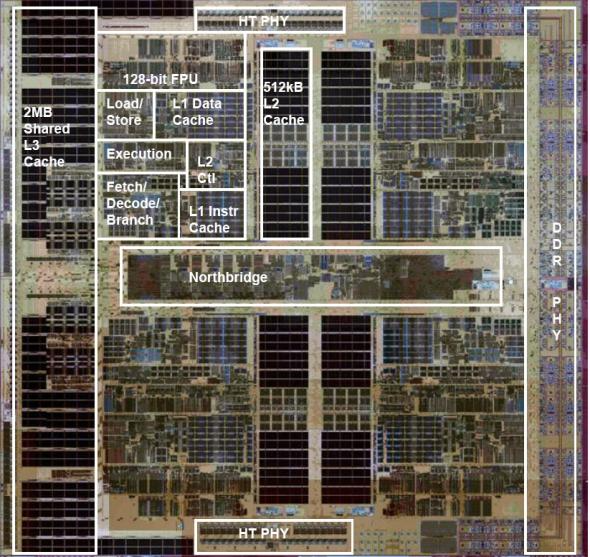
\includegraphics[scale=0.4]{images/amd_barcelona_die.png}
\end{center}

\section{Instructions: Language of the Computer}

To command a computer you must speak its language. The words of a computer language are called \textit{instructions}, and its vocabulary called an \textit{instruction set}. The \textit{stored-program concept} is the idea that instructions and data of many types can be stored in a computer's memory as numbers.

\subsection{Instructions for Making Decisions}

\textit{Conditional branch} instructions are analogous to \verb|if| and \verb|goto| statements in a programming language e.g. the following ``branch if equal'' instruction
\begin{center}
    \verb|beq register1, register2, L1|
\end{center}
goes to the statement labeled \verb|L1| if the value in \verb|register1| and \verb|register2| are equal.


\section{Arithmetic for Computers}

Addition, substraction, multiplication, division, floating point, ALU, etc.

\section{The Processor}

To understand the basics of a processor implementation, we can look at the construction of the datapath and control path for an implementation of the MIPS instruction set. This includes a subset of the core MIPS instruction set:
\begin{itemize}
    \item The memory reference instructions load word (\verb|lw|) and store word (\verb|sw|)
    \item The arithmetic-logical instructions \verb|add|,\verb|sub|,\verb|AND|,\verb|OR|, and \verb|slt|
    \item The instructions branch equal (\verb|beq|) and jump(\verb|j|)
\end{itemize}

Overall, much of what needs to be done to implement these instructions is the same regardless of the exact class of instruction. For every instruction, the first two steps are identical:
\begin{enumerate}
    \item Send the program counter (PC) to the memory that contains the code and fetch the instruction from that memory.
    \item Read one or two registers, using fields of the instruction to select the registers to read. 
\end{enumerate}
For example, the diagram below shows a high level, abstract outline of a MIPS processor implementation.
\begin{center}
    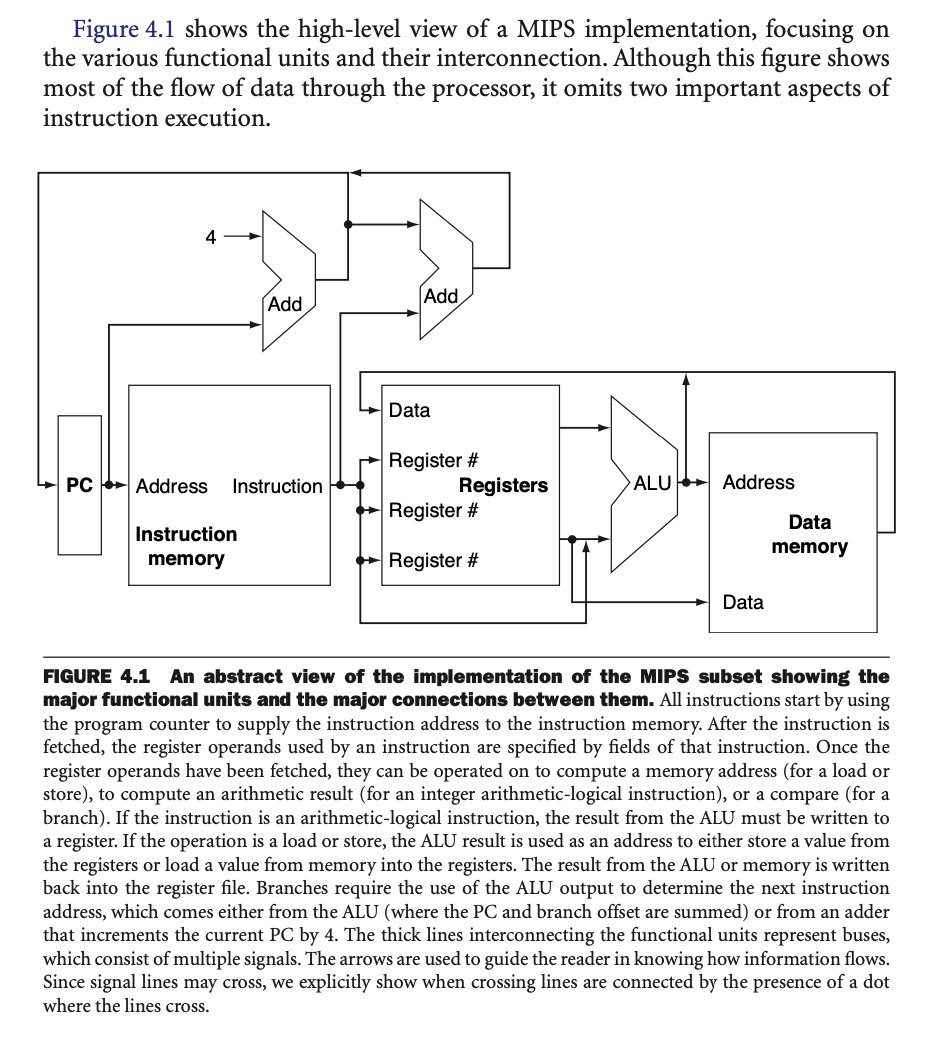
\includegraphics[scale=0.45]{images/mips_processor_high_level.png}
\end{center}

\subsection{Logic Design Conventions}

Note that the datapath elements of a MIPS implementation consists of two different type of logic elements:
\begin{itemize}
    \item \textbf{Combinational}: elements that operate on data values, where their outputs always depend only on the current inputs (i.e. think of them as implementing pure functions)
    \item \textbf{Sequential}: elements that contain some internal \textit{state}. These elements have at least two inputs and one output, where the inputs are:
    \begin{enumerate}
        \item The data value to be written.
        \item The clock.
    \end{enumerate}
    The output from a sequential logic component provides the value that was written in an earlier clock cycle.
\end{itemize}
A \textit{clocking methodology} defines when signals can be read and when they can be written. We can assume an \textit{edge-triggered clocking} methodology, which means that any values stored in a sequential logic element are updated only on a clock edge. 

Since state (i.e. sequential) elements are the only ones that can store values, any collection of combinational logic must have its inputs come from a set of state elements and its outputs written into a set of state elements The inputs are values that were written in a previous clock cycle, while the outputs are values that can be used in a following clock cycle.

\subsection{Pipelining}

TODO.

\section{The Memory Hierarchy}

In an ideal world, we would have an infinitely large and fast memory for our computer, but this is not feasible in practice, since fast memory is costly. So, instead, we simulate the illusion of an infinite memory by using a \textit{memory hierarchy}. Essentially, a progressively larger and slower series of caches that serve as memory for the processor.

\begin{center}
    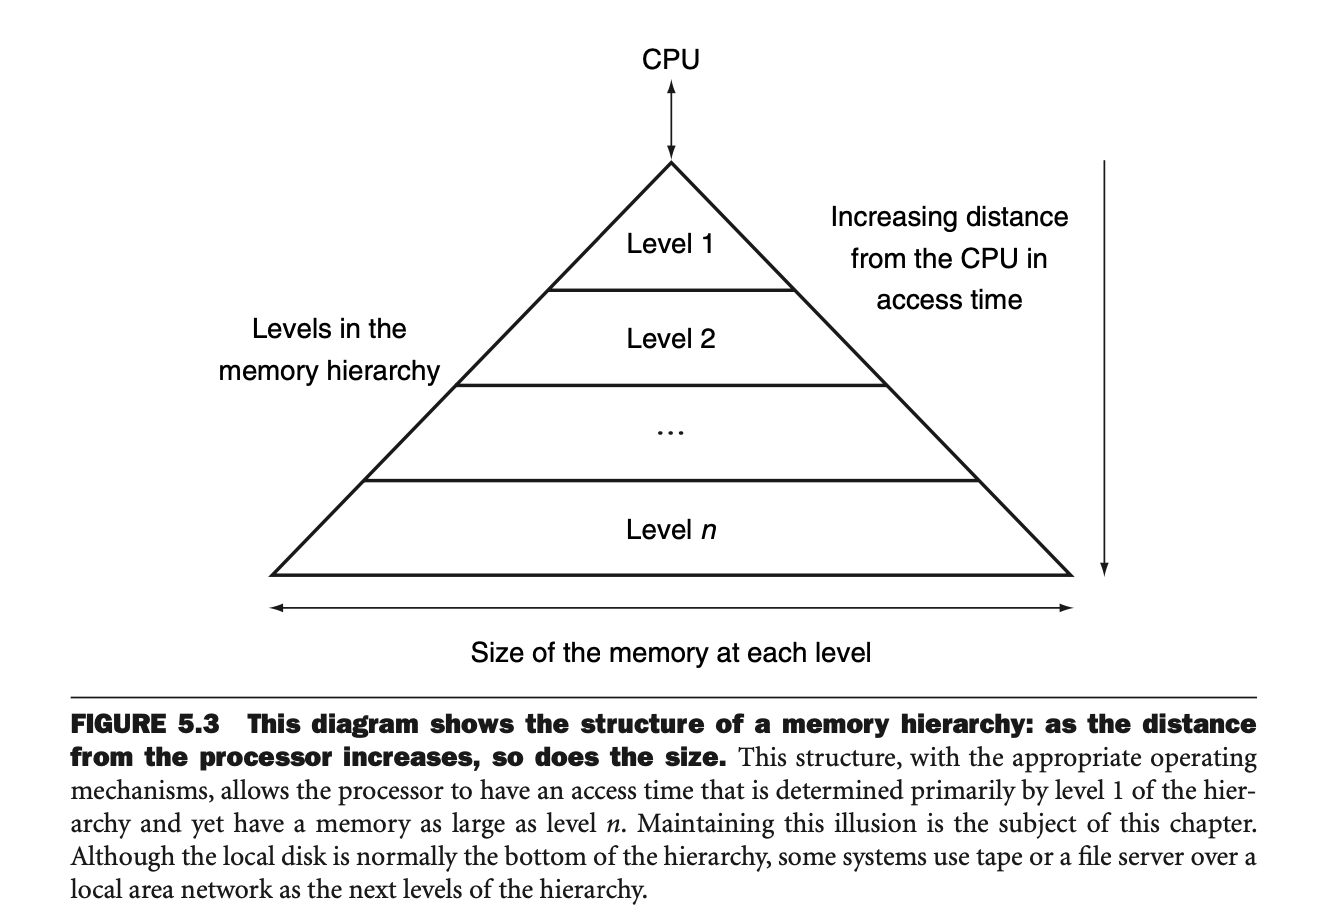
\includegraphics[scale=0.35]{images/memory_levels.png}
\end{center}

\bibliographystyle{plain}
\bibliography{../../references.bib}

\end{document}